%%
\documentclass[12pt, letterpaper]{article}
%%Packages
\usepackage{parskip}
\usepackage{url}
\usepackage{graphicx}
\usepackage{caption}
\usepackage{subcaption}
\usepackage{listings}
\usepackage{float}
\usepackage{xcolor}
\usepackage{hyperref}
\hypersetup{
    colorlinks,
    citecolor=black,
    filecolor=black,
    linkcolor=black,
    urlcolor=black
}
\graphicspath{{img/}}

\definecolor{commentgreen}{RGB}{2,112,10}
\definecolor{eminence}{RGB}{108,48,130}
\definecolor{weborange}{RGB}{255,165,0}
\definecolor{frenchplum}{RGB}{129,20,83}

\lstset{
    language=C,
    frame=tb,
    tabsize=2,
    showstringspaces=false,
    numbers=left,
    upquote=true,
    commentstyle=\color{commentgreen},
    keywordstyle=\color{eminence},
    stringstyle=\color{red},
    basicstyle=\small\ttfamily,
    emph={int,char,double,float,unsigned,void,bool},
    emphstyle={\color{blue}},
    escapechar=\&,
    classoffset=1, 
    morekeywords={>,<,.,;,,,-,!,=,~},
    keywordstyle=\color{weborange},
    classoffset=0,
    captionpos=b,
    breaklines=true,
    postbreak=\mbox{\textcolor{black}{$\hookrightarrow$}\space}
}
\begin{document}
\title{Informatica Grafica - Relazione Quake Engine}
\author{REDACTED 879372}
\date{Giugno 2024}
\maketitle
\tableofcontents

\section{Introduzione}

\subsection{Storia}
Nel 1996, id Software lanciò sul mercato il videogioco Quake, uno sparatutto in prima persona con un'ambientazione medievale e armi dal design futuristico. Questo titolo seguiva il successo mondiale di DOOM, un altro celebre gioco id Software che rivoluzionò i motori grafici dei videogiochi.

Prima di Quake vennero rilasciati DOOM e DOOM II, entrambi shooter che hanno rivoluzionato in modi diversi il genere e che utilizzavano uno stile grafico mista tra il bidimensionale e il tridimensionale che venne chiamato "2.5-D" il quale consisteva nell'avere delle immagini bidimensionali dette ``Sprite'' che guardano sempre verso la camera del giocatore.

John Carmack, programmatore di successo e cofondatore dell'azienda, già durante lo sviluppo di DOOM II pensava a un nuovo tipo di engine che avrebbe utilizzato una grafica 3D reale ispirato dal gioco ``Virtua Fighter'' rilasciato da Sega AM2 in quel periodo.

Una delle caratteristiche chiave dell'aspetto di grafico di Quake era appunto l'uso di poligoni realmente 3D per rappresentare ogni elemento visivo. Questo approccio permetteva tecniche avanzate di illuminazione e shading, creando effetti di luce dinamica e ombre più realistiche, migliorando molto l'aspetto visivo e la percezione dello spazio non che la velocità di rendering. \cite{laidlaw_1996}

Dopo la pubblicazione di DOOM II, l'idea di ``QUAKE'' girava già da tempo, inizialmente il nome doveva essere il protagonista di un videogioco ``The Fight for Justice'' che venne annunciato come pubblicità all'interno della trilogia di ``Commander Keen'' (gioco del 1990 sempre di id Software) ma che non venne mai rilasciato. 

Quando venne ideata la prima bozza di Quake il protagonista si sarebbe dovutoispirare al mito pagano di Thor e doveva trattarsi di un gioco di ruolo come quelli che esistevano in quel periodo solo più cupo e violento, lo stile grafico doveva avere varie sezioni in stili diversi tra cui una con lo stile mesoamericano azteco, ma nonostante le texture fossero già state disegnate da Adrian Carmack vennero successivamente scartate e si optò per uno stile medievale nello stile dei racconti di Lovecraft.

John Carmack lavorò al motore grafico di Quake giorno e notte 80 ore alla settimana e durante lo sviluppò pubblicò in uno pseudo-blog tramite file ".plan'' la lista delle cose a cui stava lavorando di volta in volta. Tra le problematiche principali che rallentarono il suo lavoro ci furono la questione della determinazione delle superfici visibili e l'ottimizzazione del codice.

Per farsi aiutare John Carmack assunse temporaneamente il programmatore Microsoft Michael Abrash specializzato in grafica e ottimizzazione assembly, quest'ultimo descrisse lo sviluppo di Quake all'interno del Dr. Dobb Journal in diversi articoli che verranno poi rilasciati sotto forma di libro nel \texttt{Graphics Programming Black Book} del 1997. \cite{abrash1997michael}

John Romero, lead-designer eccentrico anch'esso co-fondatore, aveva un'idea molto generica e approssimata di quello che sarbbe dovuto essere il design del gioco, il che causò una discussione con gli altri fondatorì che portò quest'ultimo a lasciare l'azienda dopo il rilascio del gioco, motivo per il quale lo stile di Quake non è molto diverso dai giochi precedenti.

Alla fine dello sviluppo del'engine, l'intero team era esausto e non riusciva a trovare idee originali per il gioco. L'idea di Romero venne scartata a favore di un gioco più simile a DOOM che si sapeva avrebbe avuto un mercato migliore. Sebbene l'ambientazione medievale venne mantenuta, i vari designer adottarono stili molto diversi, mescolando elementi medievali, gotici, militari e futuristici. Le differenze stilistiche dei vari livelli e la loro sconnessione venne giustificata a livello di storia tramite gli ``slipgate'' che si trovano a inizio e fine di ogni livello, questi portali trasportano il protagonista attraverso diverse epoce storiche e diversi luoghi.
\cite[Chapter~12]{kushner2004masters}

Fin dal rilascio vennero resi disponibili strumenti per estendere il gioco, tra cui un compilatore per il linguaggio \texttt{QuakeC} creato apposta per aggiungere nemici, armi e modalità di gioco il cui codice viene compilato in bytecode all'interno di file \texttt{progs.dat} condivisibili e diversi strumenti per la creazione di mappe di gioco tra cui \texttt{qBSP}.

Il codice sorgente venne rilasciato nel 1999 sotto licenza GPL \cite{idsoftware:quake} permettendo a diversi sviluppatori di creare modifiche o giochi nuovi tra cui ``TeamFortress'' e l'engine \texttt{GoldSrc} del gioco ``Half Life''.

\begin{figure}[H]
\centering
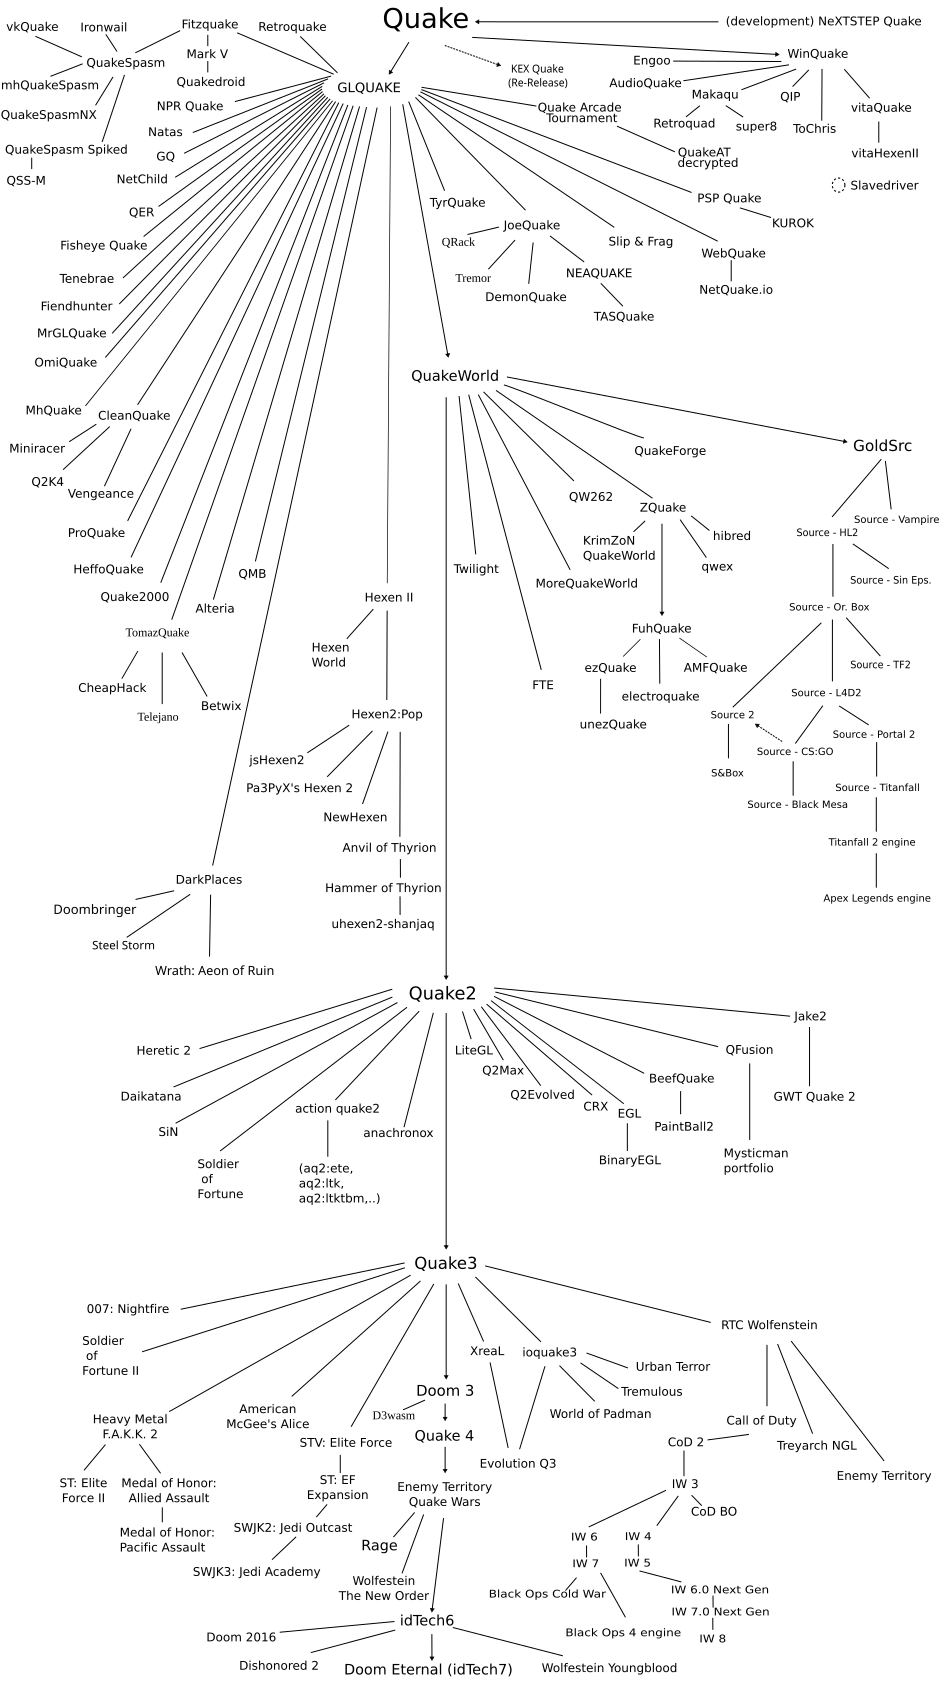
\includegraphics[width=0.75\textwidth]{quake_family_tree}
\caption { Albero che mostra tutte le derivazioni del Quake Engine \cite{enwiki:1221977912}}
\label{fig:Quake Family Tree}
\end{figure}

\subsection{Come si presenta il gioco}
Il gioco presenta una modalità per giocatore singolo in cui bisogna attraversare labirinti e sconfiggere mostri di varie forme. Include texture animate, luci statiche e dinamiche ed effetti particellari semplici, ma nella sua versione originale non implementa ombre dinamiche né illuminazione a colori. I modelli 3D sono molto semplici e le animazioni non sono interpolate, l'aspetto varia radicalmente in ogni port del motore di gioco.

%%Migliorare questa parte

\begin{figure}[H]
\centering
\begin{subfigure}[b]{0.49\textwidth}
  \centering
  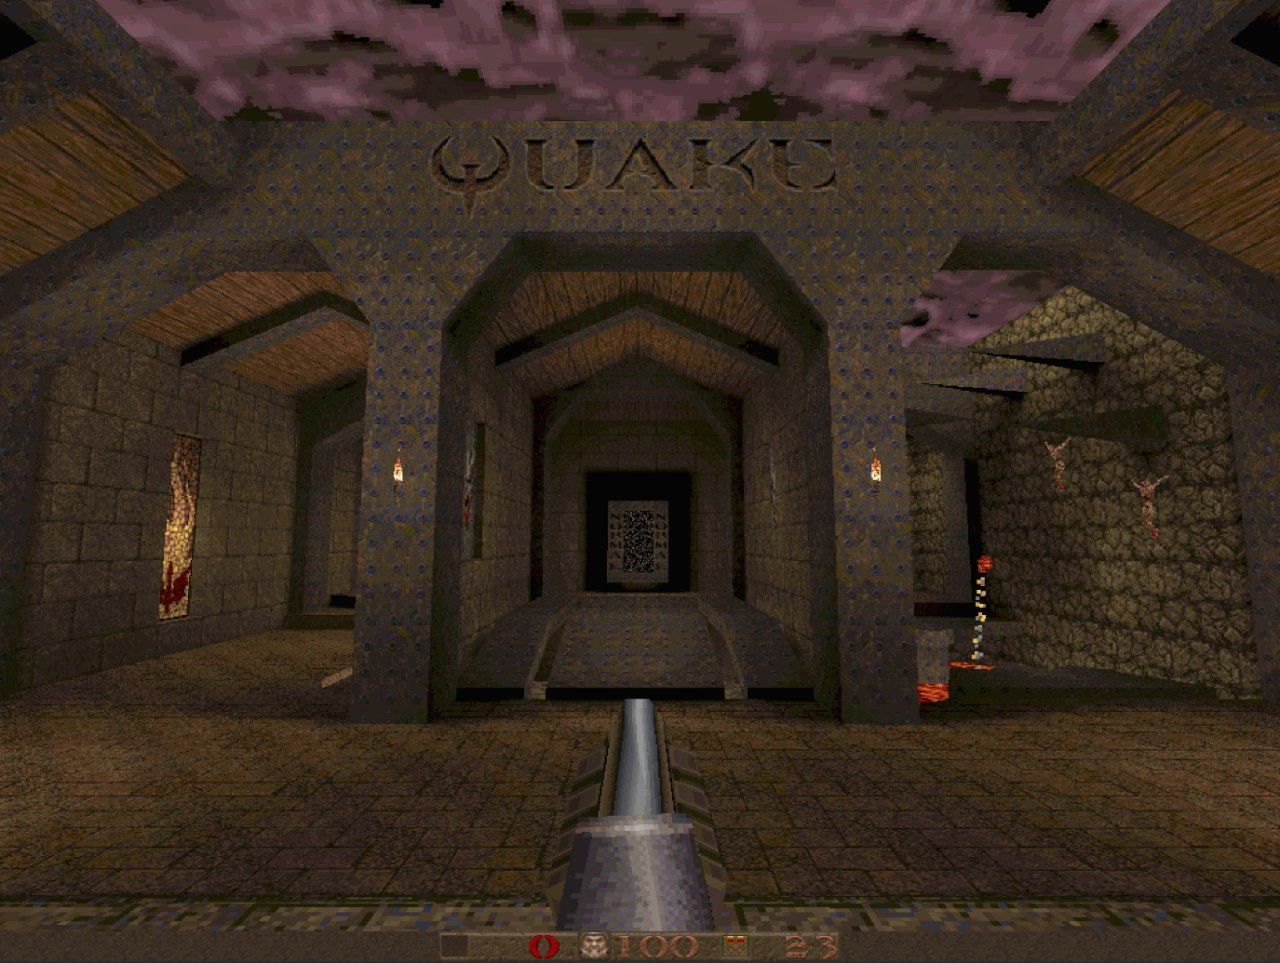
\includegraphics[width=\textwidth]{DOSBox-Quake}
  \caption{ Versione originale di Quake su emulatore DOSBox}
  \label{fig:DOSBox Quake}
\end{subfigure}
\hfill
\begin{subfigure}[b]{0.49\textwidth}
  \centering
  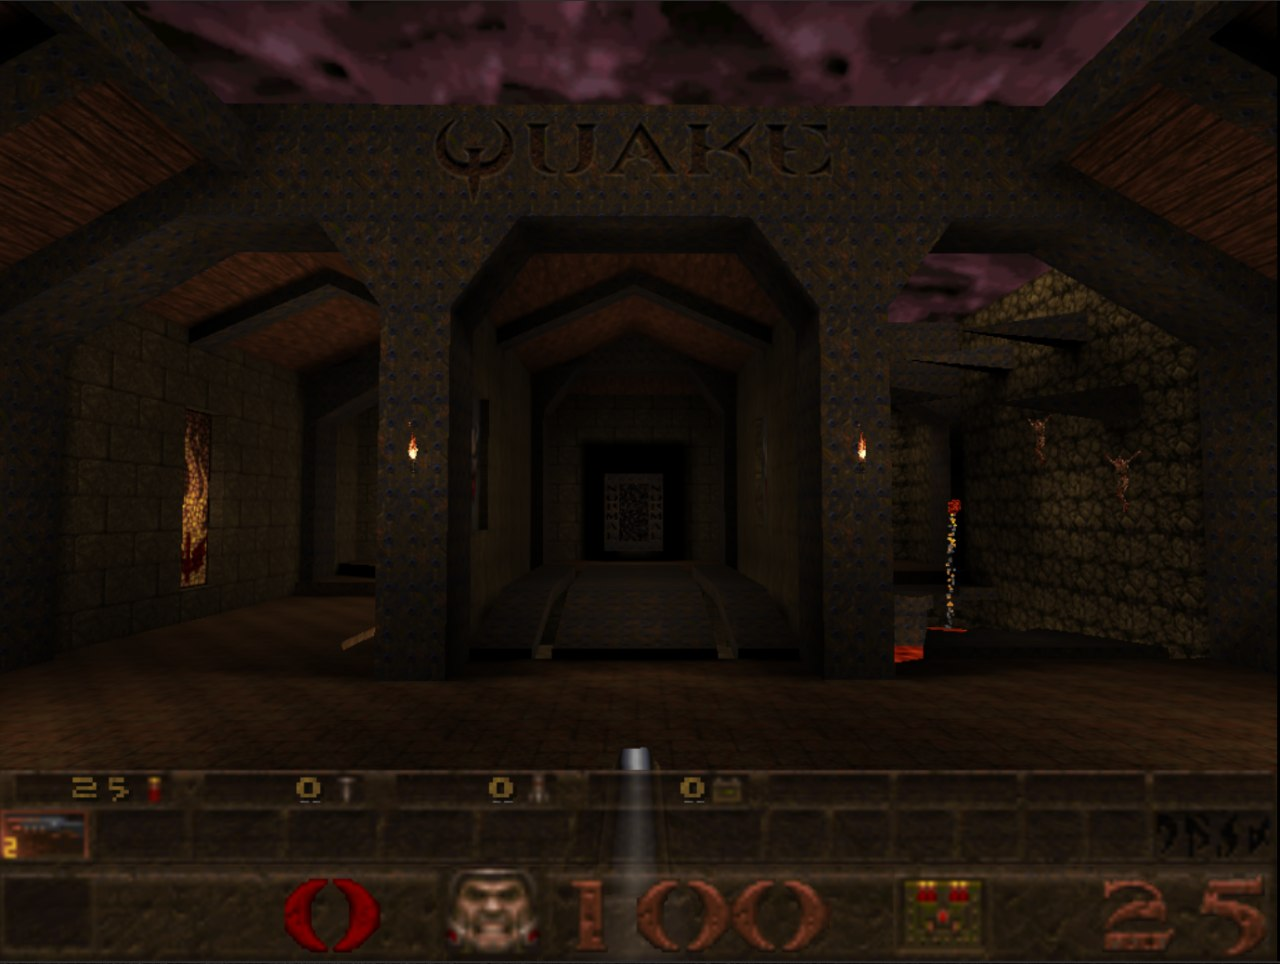
\includegraphics[width=\textwidth]{Darkplaces-Quake}
  \caption{Engine QuakeSpasm su un sistema moderno}
  \label{fig:Darkplaces Quake}
\end{subfigure}
\caption{Comparazione tra due diverse versioni del Quake Engine.}
\label{fig:Quake comparison}
\end{figure}

Una versione successiva chiamata \texttt{Quake World} invece da la possibilità di collegarsi ad altri giocatori tramite LAN o internet in una modalità ``Deathmatch'' a 8 giocatori simile a quella di \texttt{DOOM II}.  

\section{Visible Surface Determination}
\label{vsd}
\subsection{Binary Space Partitioning}
Un elemento comune tra \texttt{DOOM}, \texttt{Quake} e \texttt{Half-Life} è che tutti e tre i giochi sono prevalentemente ambientati in spazi chiusi con labirinti, stanze, porte e occasionalmente zone limitate dove si può vedere il cielo solo parzialmente. Questa scelta è dovuta al modo in cui i modelli 3D sono memorizzati e renderizzati nel renderer software originale, che richiedeva ottimizzazioni a causa delle limitate velocità di calcolo dei processori del periodo.

I poligoni che compongono i livelli di gioco sono memorizzati all'interno di alberi binari chiamati \texttt{Binary Space Partitioning trees (BSP)}. L'uso principale di questi alberi in Quake è limitare il disegno della geometria inutilizzata, gestire il rilevamento delle collisioni e l'audio spaziale.

Per semplificare, consideriamo un'area bidimensionale come la planimetria di una stanza. Possiamo disegnare una retta che divide questa area, ad esempio, lungo un segmento della scena, indicando quale delle due sezioni divise risultanti è da considerare ``di fronte'' alla retta (rappresentata dal nodo figlio a sinistra) e quale è dietro (rappresentata dal nodo figlio destro). Questo processo di suddivisione può essere ripetuto ricorsivamente fino a quando non sono stati utilizzati tutti i lati dei poligoni presenti.

\begin{figure}[H]
  \centering
  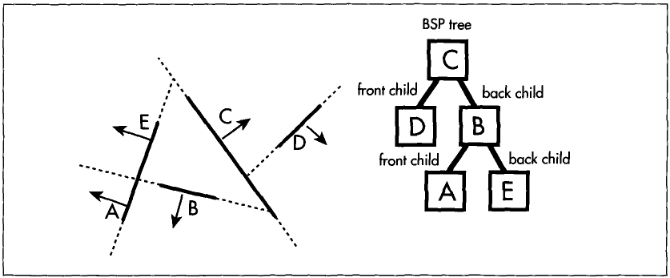
\includegraphics[width=\textwidth]{bsptree}
  \caption{Un esempio di albero BSP \cite{abrash1997michael}}
  \label{fig:Texture diff in quakes}
\end{figure}

Questo processo può essere applicato in un ambiente a tridimensionale considerando dei piani separatori al posto delle rette, la direzione frontale è data dalla direzione della normale del piano ed è possibile dimostrare che alla fine di questo processo di suddivisione tutte le foglie rappresentano sezioni del mondo convesse, le quali contengono o uno spazio ``vuoto'' (empty leaves) oppure uno spazio ``pieno'', ad esempio l'interno di un muro.
\newpage
\begin{lstlisting}[caption= Algoritmo che genera un albero BSP \cite{fuchs1980visible}]
  
Tree make_tree(polygon_list pl) {
    int k = Select_polygon(pl);
    polygon_list pos_list = null;
    polygon_list neg_list = null;
    // pos si riferisce alle parti positive
    // neg si riferisce alle parti negative
    for (int i = 0; i < Size_of(pl); i++) {
        if (i != k) {
            polygon pos_parts, neg_parts;
            Split_polygon(pl[i], pos_parts, neg_parts);
            Add(pos_parts, pos_list);
            Add(neg_parts, neg_list);
        }
    }
    
    return Combine_tree(make_tree(pos_list),
                        pl[k], make_tree(neg_list))
}
\end{lstlisting}

Per determinare in che foglia si trova un punto del mondo si parte dalla radice dell'albero BSP e si verifica se il punto in questione si trova davanti o dietro il piano separatore corrispondente, in base a questa decisione si percorre il sottoalbero destro o sinistro fino a quando è possibile.

L'utilita di questa struttura dati sta nel fatto che è molto semplice percorrere l'albero per ottenere un ordinamento delle foglie in base alla distanza tramite degli algoritmi di visita, ciò viene utilizzato per la determinazione delle superfici visibili in quanto la visita \texttt{in-order} di questo albero, troncata quando viene trovata la locazione del punto di vista permette di ottenere tutti i poligoni in ordine dal più lontano al più vicino ad essa (back-to-front).

Un algoritmo di disegno comune utilizzabile con gli alberi BSP è il \texttt{Painter's Algorithm} che consiste nel disegnare i poligoni in ordine dal più lontano al più vicino appunto sfruttando la visita back-to-front. Sebbene sia semplice da implementare, il \texttt{Painter's Algorithm} non è ottimale poiché causa un notevole overdraw, cioè il ridisegno di pixel che vengono successivamente coperti da altri poligoni.\newpage


\begin{lstlisting}[caption=Un algoritmo di visita in-order (Back-To-Front)  \cite{fuchs1980visible}]
void Back_to_front(viewing_position eye, BSP_tree t) {
    if (t != NULL) {
        if (pos_side_of(t->root, eye)) {
            Back_to_front(eye, t->neg_branch);
            Visit(t->root);
            Back_to_front(eye, t->pos_branch);
        } else {
            Back_to_front(eye, t->pos_branch);
            Visit(t->root);
            Back_to_front(eye, t->neg_branch);
        }
    }
  }
\end{lstlisting}

L'engine di Quake utilizza alberi BSP per rappresentare tutta la geometria dei livelli di gioco, a differenza di altre implementazioni, i poligoni non sono memorizzati all'interno dei nodi dell'albero come parte dei piani di divisione, ma sono invece collocati nelle foglie vuote. Poiché queste foglie rappresentano regioni convesse, i poligoni si trovano sui confini di questi spazi e sono orientati sempre verso l'interno, assicurando che nessun poligono possa oscurarne un altro (proprietà dei poliedri convessi) \cite{abrash1997michael}.

Un'altra differenza importante è che Quake utilizza un ordine di rendering front-to-back, quindi inverte l'ordine rispetto a quello di visita. Questo approccio, che verrà spiegato in dettaglio successivamente, aiuta a migliorare l'efficienza del rendering riducendo il numero di poligoni ridisegnati.

Un livello di Quake è memorizzato in un file .BSP compilato tramite il tool qBSP, che prende in input un file testuale .MAP generato dal designer tramite un software CAD apposito come per esempio \texttt{TrenchBroom}, questi software usano la geometria solida costruttiva tramite dei ``brush'' e possono rappresentare sia elementi strutturali, utilizzati per la determinazione delle superfici visibili, che elementi di dettaglio che vengono rimossi durante la fase di ottimizzazione.

Questo file non contiene solo l'albero BSP, ma anche informazioni sulle entità, le texture di gioco, l'illuminazione, le liste di visibilità e altre informazioni utili per velocizzare il rendering, il quale viene calcolato off-line.
\newpage

\begin{lstlisting}[caption=Nodi dell'albero BSP all'interno di \texttt{bspfile.h} \cite{idsoftware:quake}]
  typedef struct {
    int			planenum;
    short		children[2]; 
  } dclipnode_t;
  extern	int			numclipnodes;
  extern	dclipnode_t	dclipnodes[MAX_MAP_CLIPNODES];

\end{lstlisting}


\begin{lstlisting}[caption=Funzione \texttt{SV\_HullPointContents} all'interno di \texttt{world.c} \cite{idsoftware:quake} che trova la foglia in cui è contenuto un punto p. ]
  int SV_HullPointContents (hull_t *hull, int num, vec3_t p)
{
	float		d;
	dclipnode_t	*node;
	mplane_t	*plane;

	while (num >= 0)
	{
		if (num < hull->firstclipnode || num > hull->lastclipnode)
			SV_Error("SV_HullPointContents: bad node number");
	
		node = hull->clipnodes + num;
		plane = hull->planes + node->planenum;
		
		if (plane->type < 3)
			d = p[plane->type] - plane->dist;
		else
			d = DotProduct (plane->normal, p) - plane->dist;
		if (d < 0)
			num = node->children[1];
		else
			num = node->children[0];
	}
	
	return num;
}
  \end{lstlisting}

\subsection{Frustum Clipping e Potentially Visible Sets}

Il principale ostacolo che John Carmack dovette affrontare durante lo sviluppo del gioco fu l'overdraw eccessivo causato dall'utilizzo di algoritmi come il \texttt{Painter's Algorithm}, il quale in scenari complessi disegnava più di dieci volte la geometria necessaria, con conseguente degrado significativo delle prestazioni.

Un primo approccio per mitigare l'overdraw consiste nell'esaminare l'albero BSP e tagliare fuori tutti i nodi che si trovano al di fuori del frustum di vista (frustum culling). In questo modo, la maggior parte dei poligoni può essere esclusa quasi istantaneamente.

La soluzione adottata da Carmack per diminuire ulteriormente la geometria da renderizzare consiste nel calcolo di un \texttt{Potentially Visible Set (PVS)} per ogni foglia, ovvero una lista che include tutte le foglie visibili da qualsiasi punto all'interno di una foglia. Calcolare questa lista richiedeva un tempo considerevole, per esempio tra i 10 e i 30 minuti su un processore Alpha \cite{abrash1997michael} e quindi veniva sempre eseguito durante la compilazione della mappa piuttosto che a runtime.

Per implementare i PVS, è necessario partire da un \texttt{portal graph}. Ogni coppia di foglie vuote confinanti implica l'esistenza di un poligono vuoto che li collega, questo poligono è chiamato \texttt{portale} e rappresenta il percorso che va attraversato per passare da una foglia all'altra. Questi portali vengono estratti dal compilatore e associati alle rispettive foglie, dando vita a una struttura a grafo avente le foglie come nodi e i portali come lati, chiamato appunto \texttt{portal graph}.

\begin{figure}[H]
  \centering
  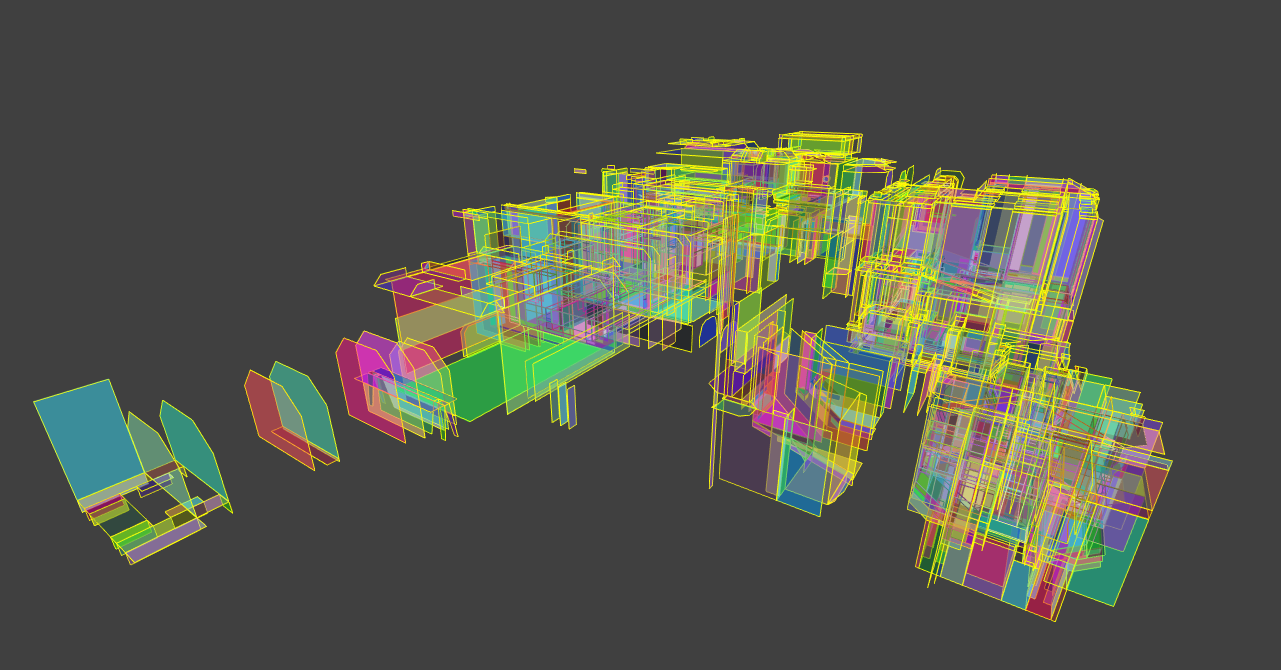
\includegraphics[width=\textwidth]{portals}
  \caption{Visualizzazione dei portali nel map editor NetRadiant}
  \label{fig:Texture diff in quakes}
\end{figure}

A partire da una foglia e una delle foglie che si trovano davanti ad essa l'obiettivo è capire se esiste un segmento che collega la prima con quella di arrivo senza passare attraverso zone solide, ciò equivale a dire che il segmento deve passare solo attraverso dei portali.

Per capire se un portale è visibile da un altro quando si attraversano più foglie il compilatore utilizza dei separatori, un separatore è un piano che viene fatto passare per ogni segmento del portale di partenza e tocca il portale della foglia successiva dal lato opposto, questo separatore ha una direzione definita dalla sua normale; con questa informazione è possibile tagliare un terzo portale che incontra eliminando tutti i punti che si trovano dietro al separatore in quanto non sono visibili, se il portale viene tagliato interamente allora la foglia che raggiunge viene rimossa e il processo si ferma.

\begin{figure}[H]
  \centering
  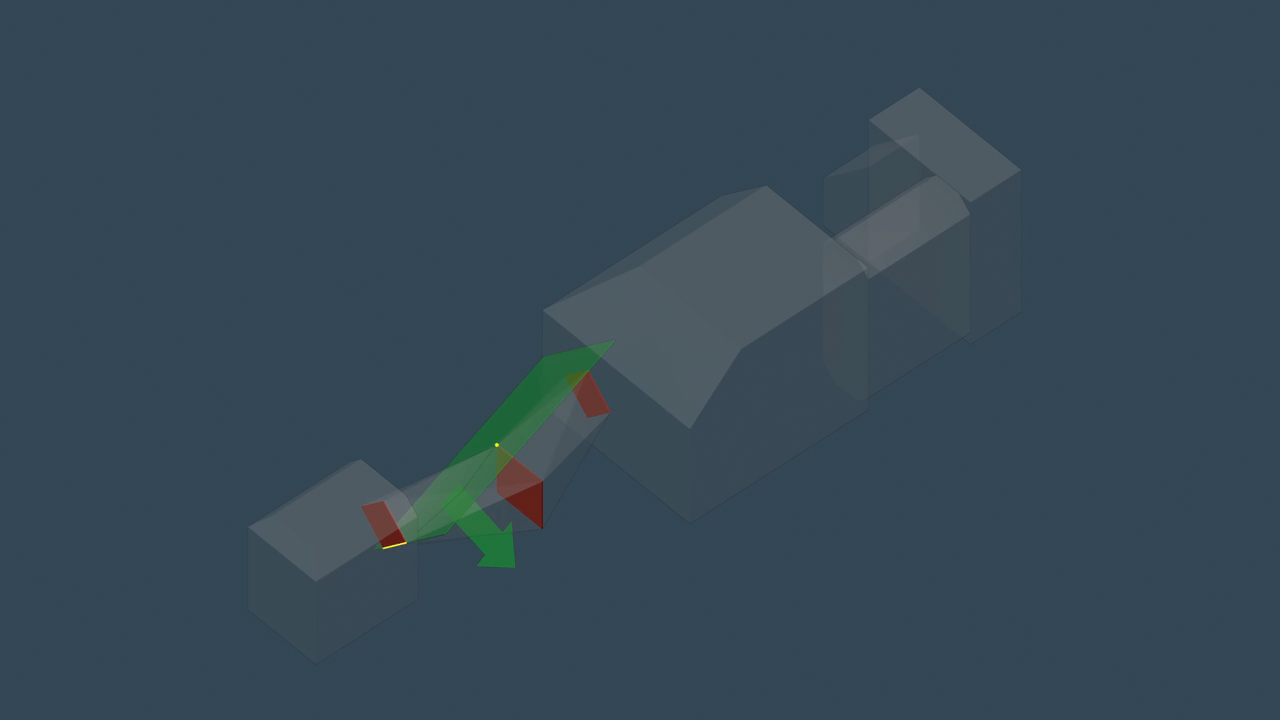
\includegraphics[width=\textwidth]{MattRamblings_Portals}
  \caption{Esempio di piano separatore che passa per tre portali \cite{matt2023quakepvs} }
  \label{fig:Texture diff in quakes}
\end{figure}

Quando si tratta di tre portali allineati, è possibile calcolare la visibilità con precisione assoluta. Tuttavia, quando si hanno quattro o più portali non è possibile calcolare la visibilità con certezza, poiché il processo per determinare la visibilità in modo accurato è molto più complesso \cite{nirenstein2002exact}.

Per semplificare i calcoli necessari, Quake adotta un'approccio conservativo, esegue il clipping dei portali in gruppi di tre lungo il percorso che va dal portale di partenza al portale di destinazione. Questo processo procede ricorsivamente, con ciascun portale che viene tagliato basandosi su quello che è stato tagliato precedentemente. Ogni linea che attraversa tutti i portali intermedi deve necessariamente passare attraverso tutti e tre portali considerati, il che porta all'assegnazione del marchio di "visibilità" a ogni foglia visibile.

\begin{figure}[H]
  \centering
  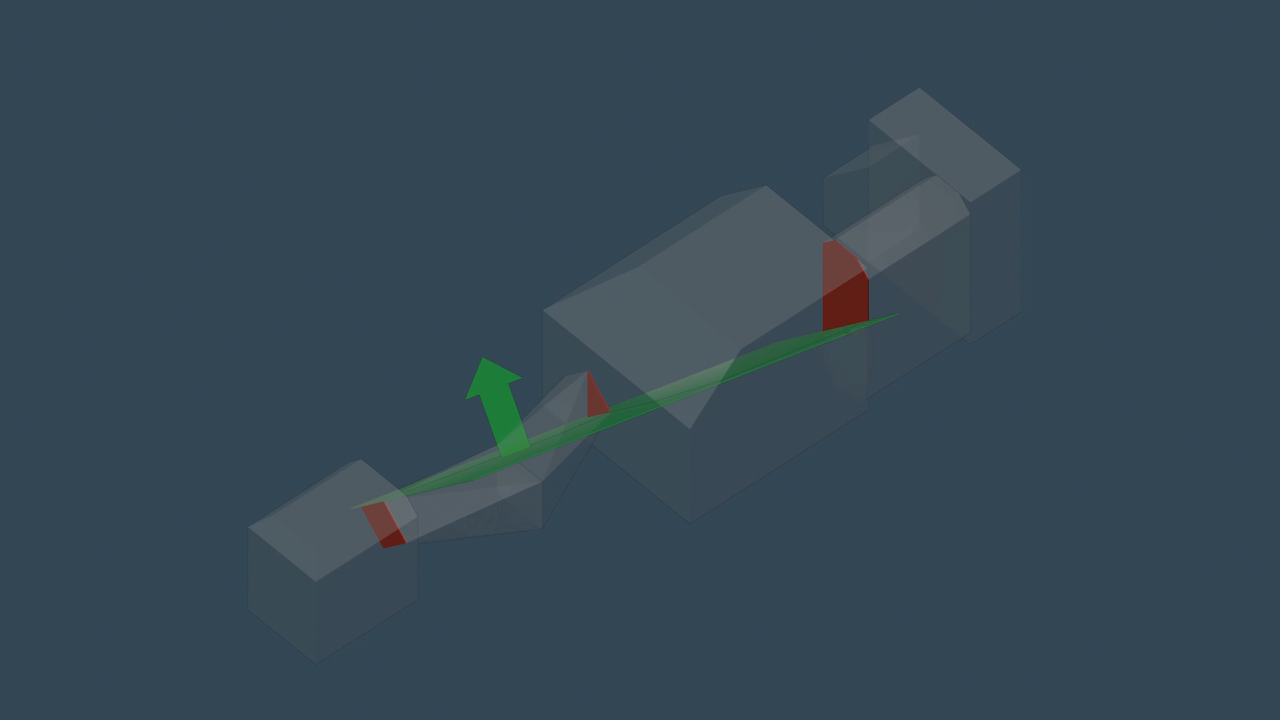
\includegraphics[width=\textwidth]{MattRamblings_Portals_2}
  \caption{Esempio di piano separatore che passa per tre portali non consecutivi e taglia un terzo portale \cite{matt2023quakepvs} }
  \label{fig:Texture diff in quakes}
\end{figure}

Tuttavia, è importante notare che possono esistere linee che attraversano questo gruppo ristretto di portali ma non tutti quelli intermedi, causando l'assegnazione del marchio di "visibilità" a foglie che non sono visibili, da qui l'uso dell'avverbio "Potenzialmente".

Questo processo può essere applicato all'intero grafo dei portali tramite una ricerca ricorsiva depth-first attraverso ogni possibile sequenza di portali la quale termina appena viene incontrata una foglia non visibile. \cite{matt2023quakepvs}

Ulteriori ottimizzazioni permettono di comprimere il PVS, ad esempio per il livello \texttt{E1M1} questo insieme compone intorno al 3\% del file .bsp compilato e occupa 40 kilobytes su disco.

\begin{figure}[H]
  \centering
  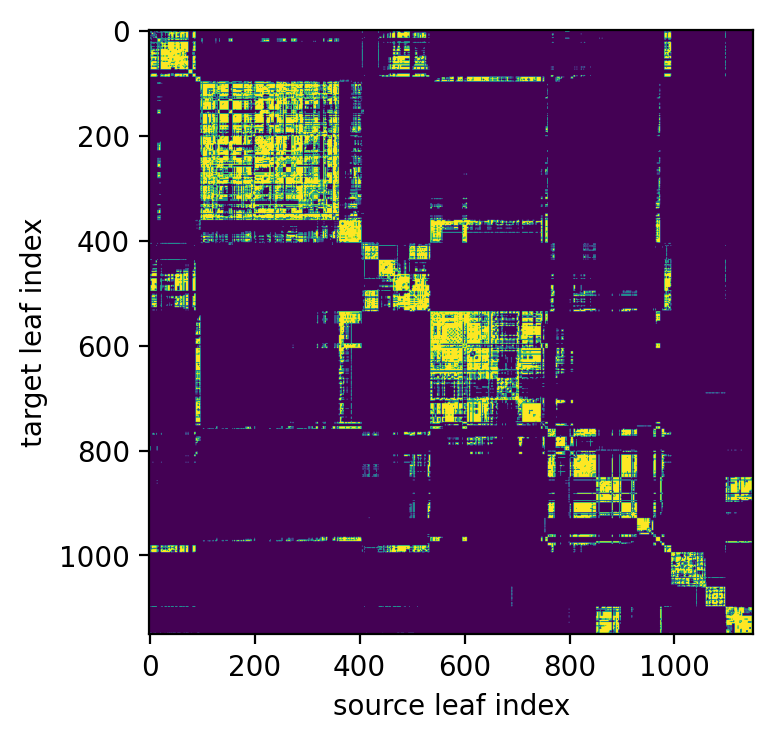
\includegraphics[width=\textwidth]{MattRamblings_PVS_2D}
  \caption{Visualizzazione in un'immagine bidimensionale della bitmap riguardante il PVS di ogni foglia all'interno del livello E1M1 \cite{matt2023quakepvs}}
  \label{fig:Texture diff in quakes}
\end{figure}

\newpage

\subsection{Hidden Surface Removal}

Nonostante fossero state apportate ottimizzazioni, il Potentially Visible Set (PVS) conteneva mediamente circa cinque volte più poligoni di quelli visibili. Questo in aggiunta all'utilizzo del rendering Back-To-Front con il Painter's Algorithm comportava un rallentamento delle performance non ideale. Per risolvere questo problema venne sviluppata un'ulteriore ottimizzazione: \texttt{lo span-sorting}.

\begin{figure}[H]
  \centering
  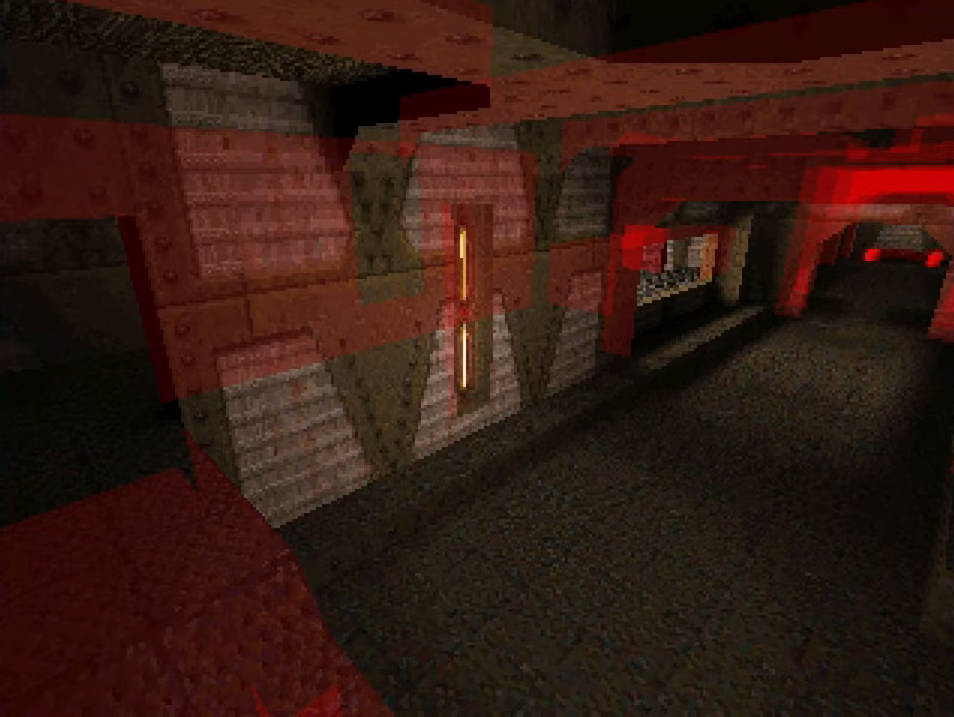
\includegraphics[width=\textwidth]{MattRamblings_OverDraw}
  \caption{In rosso l'overdraw causato dal Painter's Algorithm \cite{matt2023quakehsr}}
  \label{fig:Texture diff in quakes}
\end{figure}


Lo span-sorting opera suddividendo ogni poligono, visitati in ordine Front-To-Back, in linee orizzontali di pixel (span), rappresentati dal loro punto di inizio sull'asse x, la y di cui fa parte l'intera linea e la lunghezza. Queste linee vengono successivamente ordinate e ridotte fino a che non restano solo le sezioni visibili.

Rispetto allo z-buffering, che valuta i singoli pixel, lo span-sorting focalizza l'attenzione sulle sovrapposizioni tra queste linee orizzontali (span), portando a un significativo miglioramento nelle performance del processo di rendering.

Per generare gli span vengono inizialmente generati tutti gli spigoli per ogni poligono nel frustum di vista, viene eseguito il clipping rispetto a quest'ultimo e infine vengono proiettati sul view plane rispetto alla camera, a questo punto viene applicato un algoritmo scanline che usa un'\texttt{Active Edge List} per ricavare gli span.

In un ambiente 3D però non è sempre chiaro quale punto è l'inizio dello span e quale è il punto finale, per questo motivo Quake memorizza un riferimento ai poligoni che si trovano sul lato destro e sinistro di ogni edge, mentre l'AEL viene aggiornata per ogni scanline da sinistra a destra, mantiene anche una Active Polygon List, ogni volta che viene incontrato uno spigolo il poligono di sinistra viene rimosso dalla APL e il poligono di destra è aggiunto all'APL, questa lista è a sua volta ordinata rispetto alla distanza dalla camera utilizzando l'ordine in cui la superficie è stata incontrata all'interno dell'albero BSP come chiave, quando il poligono che si trova in cima alla lista cambia, lo span del vecchio poligono che stava in cima finisce e quello successivo viene creato. \cite{matt2023quakehsr}

Una volta che gli span sono stati calcolati i poligoni vengono attraversati uno alla volta e gli span di ogni poligono vengono rasterizzati, rimuovendo completamente la necessità di sovrascrivere i pixel.



\begin{figure}[H]
  \centering
  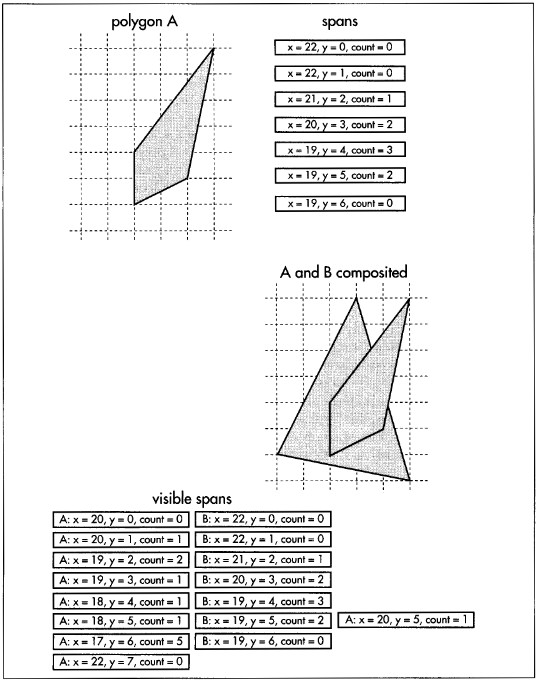
\includegraphics[width=\textwidth]{sortedspans}
  \caption{Clipping di due span sets ordinati \cite{abrash1997michael}}
  \label{fig:Texture diff in quakes}
\end{figure}



\subsection{Moving Entities}

Esistono tre tipi di entità all'interno dell'engine di Quake. Il primo consiste nei modelli BSP, i quali rappresentano elementi della mappa di gioco che sono in grado di muoversi con dei trigger, come ponti, ascensori e porte, ma anche gli healthpack e le munizioni. Questi modelli vengono renderizzati attraverso il clipping dei loro poligoni insieme all'albero BSP, garantendo che ogni frammento si trovi in una singola foglia.

L'ordine dell'albero BSP viene sfruttato per renderizzare correttamente questi frammenti rispetto agli altri poligoni. Tuttavia, se più modelli BSP sono presenti nella stessa foglia, viene adottato un ordinamento basato sulle componenti 1/z calcolate dall'equazione del piano su cui giacciono. \cite{abrash1997michael}

Il secondo tipo di entità sono i modelli poligonali, utilizzati per rappresentare armi, mostri e altri oggetti. Per questi modelli, risulta difficile calcolare la geometria occlusa utilizzando lo stesso approccio dei livelli di gioco siccome si muovono attraverso diverse foglie dell'albero.
%% NOTA 1/z è la pseudodepth, lo usiamo perchè varia linearmente e perchè permette l'interpolazione prospettivamente corretta come per le texture TODO: ripassa

\begin{figure}[H]
\centering
\begin{subfigure}[b]{0.49\textwidth}
  \centering
  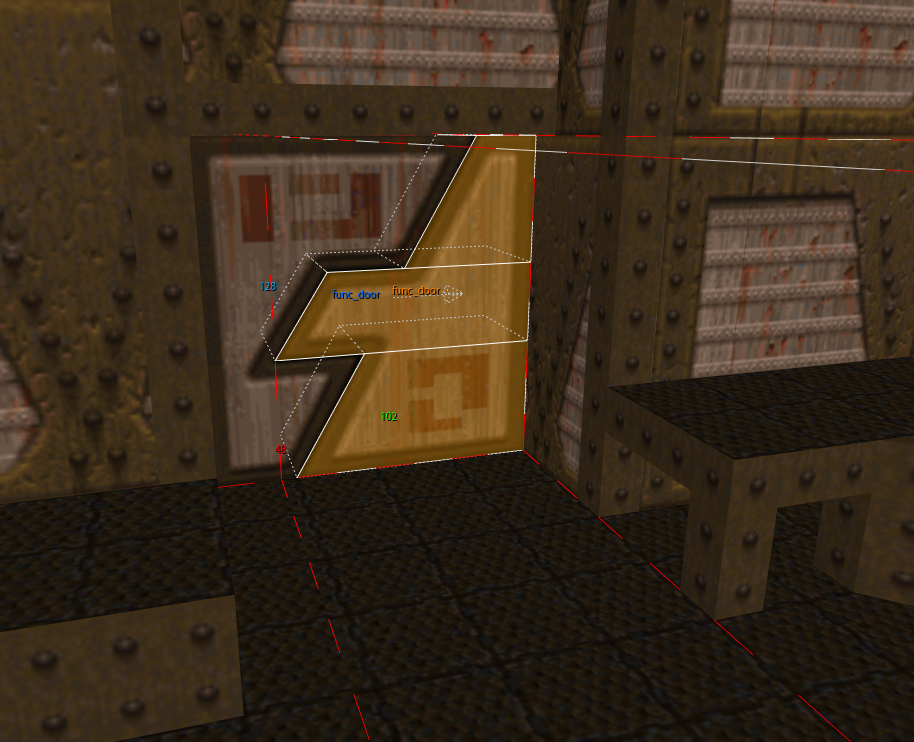
\includegraphics[width=\textwidth]{e1m1door}
  \caption{Porta E1M1}
  \label{fig:DOSBox Quake}
\end{subfigure}
\hfill
\begin{subfigure}[b]{0.49\textwidth}
  \centering
  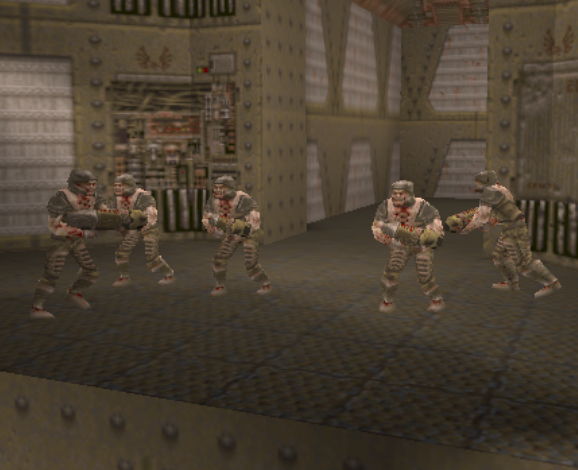
\includegraphics[width=\textwidth]{grunts}
  \caption{Nemici \emph{Grunts}}
  \label{fig:Darkplaces Quake}
\end{subfigure}
\caption{Esempi di modello BSP dinamico (a sinistra) e di modelli poligonali dinamici (a destra)}
\label{fig:Quake comparison}
\end{figure}

Dopo che gli span dei poligoni del mondo vengono disegnati viene utilizzato uno Z-Buffer solo per i modelli poligonali di questo tipo, un pixel viene disegnato solamente se la distanza della sua z è più vicina del pixel precedentemente nel buffer, questa è una soluzione low-tech utilizzata anche nel rendering hardware, che però limitava molto le performance nel rendering software, infatti Quake non supporta numerose entità di questo tipo all'interno dello spazio visibile.

Il terzo tipo di entità sono gli sprite, immagini 2D usate ad esempio per gli effetti particellari, anche questi sono renderizzati tramite l'uso di uno Z-Buffer.

\section{Lighting Model}

\subsection{Shading and Textures}

Come tecnica di shading per le entità Quake utilizza il Gouraud Shading, all'inizio viene generato un valore di illuminazione in ogni vertice applicando ogni fonte di illuminazione pertinente (descritte all'interno del file .BSP) e successivamente questi valori vengono interpolati linearmente tra tutti gli spigoli dei poligoni e poi tra ogni spigolo attraverso gli span. Il colore di ogni pixel viene quindi estratto da una texture, a cui viene applicato il valore di illuminazione per ottenere l'aspetto finale.

Le texture in Quake sono generalmente immagini di 32x32 o 64x64 pixel, una particolarità sta nel fatto che il gioco estende automaticamente tutte le texture che non hanno dimensioni pari per renderle multipli di 2, queste texture poi possono essere poi ripetute (tiling) in uno stesso poligono.

Per questioni di efficienza Quake non calcola la luce interpolata considerando le componenti RGB, che permetterebbe di avere luci colorate con un peso maggiore sulla performance, invece utilizza una color palette di 256 colori; ogni pixel è illuminato guardando una matrice chiamata \texttt{colormap} che utilizza come indici di ricerca l'intensità luminosa e il colore desiderati. Questa matrice si trova all'interno degli assets di gioco nel file \texttt{pak.PAK0} all'interno di \texttt{gfx/colormap.Imp} ed è quindi possibile modificarla.

La colormap è una tabella con 64 valori per ogni colore della palette, il numero 0 rappresenta una luminosità del 200\% (overbrightness), il 32 rappresenta il colore originale e 63 è nero, quest'ultimo è ripetuto nella matrice perchè ogni colore può essere rappresentato in ombra e risulta più comodo per i calcoli. 

\begin{figure}[H]
  \centering
  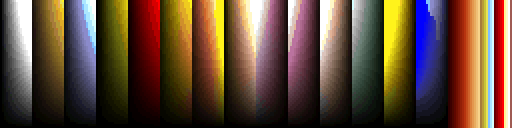
\includegraphics[width=\textwidth]{quake_color_map}
  \caption{La colormap di Quake}
  \label{fig:Texture diff in quakes}
\end{figure}

Nonostante faccia parte degli assets di gioco (i quali sono coperti da copyrights) la colormap è stata resa di dominio pubblico come la palette per facilitare il porting del gioco.

All'interno della colormap sono presenti colori denominati ``fullbright" che mantengono lo stesso colore indipendentemente dalla lightmap, apparendo sempre alla massima luminosità anche nelle sezioni in ombra. Tuttavia, poiché GLQuake non utilizza la colormap, i dettagli forniti da questi pixel vengono persi negli engine con il renderer hardware a meno che non vengono implementati con altri metodi.
\subsection{Lightmaps}

In un rasterizer software che adotta il Gouraud shading, di solito è presente una fase di pre-processing in cui vengono calcolati i valori di illuminazione per ciascun vertice. Durante l'esecuzione, questi valori possono essere aggiornati dinamicamente per gestire situazioni di illuminazione dinamiche successivamente utilizzati nel processo di shading.

Nell'approccio di Quake, invece, durante la fase di pre-processing, viene generata una struttura dati chiamata \texttt{lightmap} che viene utilizzata per definire l'illuminazione di ciascun poligono del mondo.

Ogni lightmap consiste in una griglia di valori di illuminazione assegnati a punti disposti ogni 16 pixel sia verticalmente che orizzontalmente. Per calcolare l'illuminazione, il gioco, proietta tutte le sorgenti luminose su questi punti e somma i risultati nel caso in cui sono presenti più sorgenti luminose e successivamente applica un filtro di smoothing per ottenere una transizione graduale tra i diversi livelli di illuminazione e per evitare bordi troppo definiti.

% SURFACE CACHING!

\begin{figure}[H]
\centering
\begin{subfigure}[b]{0.49\textwidth}
  \centering
  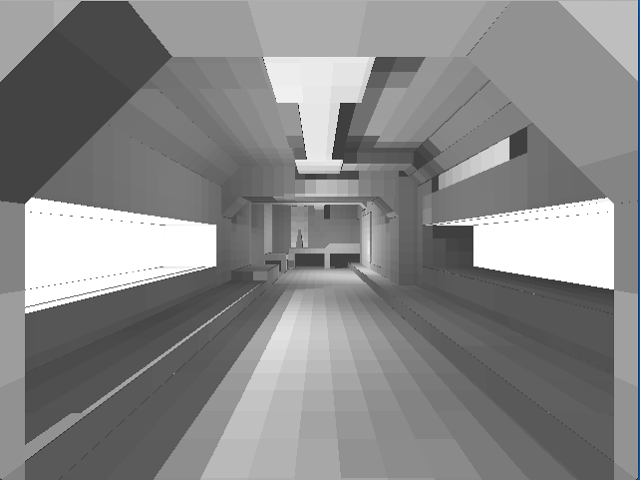
\includegraphics[width=\textwidth]{jbush_lightmap1}
  \caption{Lightmap senza smoothing}
  \label{fig:lightmap1}
\end{subfigure}
\hfill
\begin{subfigure}[b]{0.49\textwidth}
  \centering
  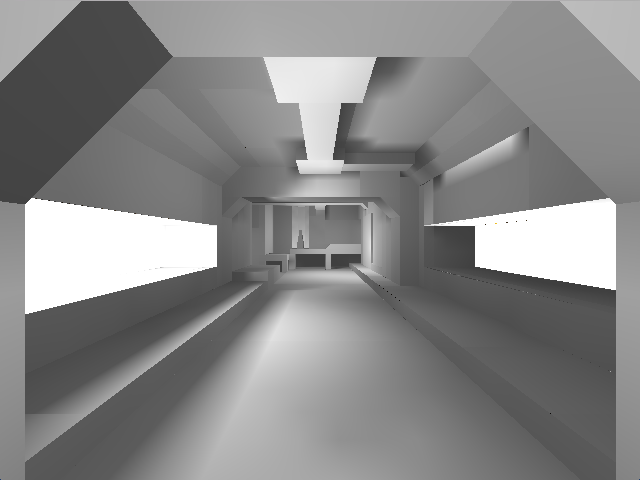
\includegraphics[width=\textwidth]{jbush_lightmap2}
  \caption{Lightmap con smoothing}
  \label{fig:lightmap2}
\end{subfigure}
\caption{Visualizzazione delle lightmaps in un livello \cite{jbush2015quakelightmaps}}
\label{fig:lightmaps comparison}
\end{figure}

Durante l'esecuzione, la texture viene inserita in un buffer in cui ogni texel è illuminato in base alla media pesata dei valori dei quattro punti della griglia della lightmap più vicini ad esso. Se è necessaria una luce dinamica, come ad esempio dopo un'esplosione, la lightmap viene aggiornata dinamicamente prima di essere inserita in questo buffer, ad esempio sommando diversi contributi luminosi. Successivamente, il poligono viene disegnato utilizzando il texture mapping prospetticamente corretto, usando questo surface buffer come texture.

%TODO: Aggiungere qualcosa????

\begin{figure}[H]
  \centering
  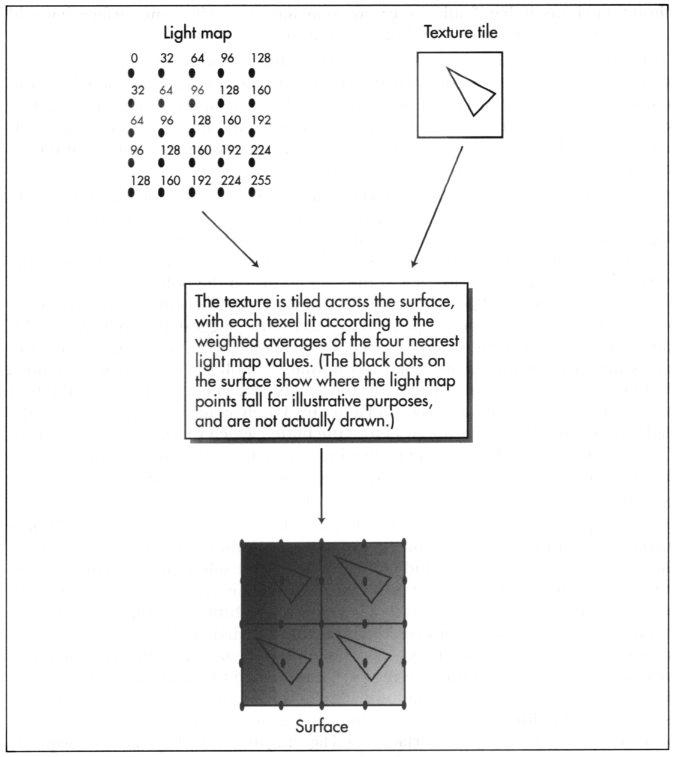
\includegraphics[width=\textwidth]{applying_lightmaps}
  \caption{Applicazione delle lightmaps \cite{abrash1997michael}}
  \label{fig:Texture diff in quakes}
\end{figure}

Poiché l'illuminazione avviene a livello di superficie anziché a screen space, questo metodo risulta corretto sia prospetticamente (a differenza del metodo tradizionale con il Gouraud Shading) che rispetto al clipping, alla rotazione e al punto di vista.

Inoltre, questo approccio consente a più luci e ombre di sovrapporsi con una risoluzione abbastanza buona. Poiché non dipende dai vertici, risolve anche i glitch grafici che si verificherebbero sulle superfici che si uniscono a T (T-junction). \cite{abrash1997michael}

Le lightmaps della geometria statica vengono pre-compilate con lo strumento \texttt{light} per ogni mappa (dopo aver rimosso i poligoni non utili a questo scopo) e aggiunte al file compilato, questo processo poteva richiedere un tempo considerevole. 

\begin{figure}[h]
\centering
\begin{subfigure}[b]{0.49\textwidth}
  \centering
  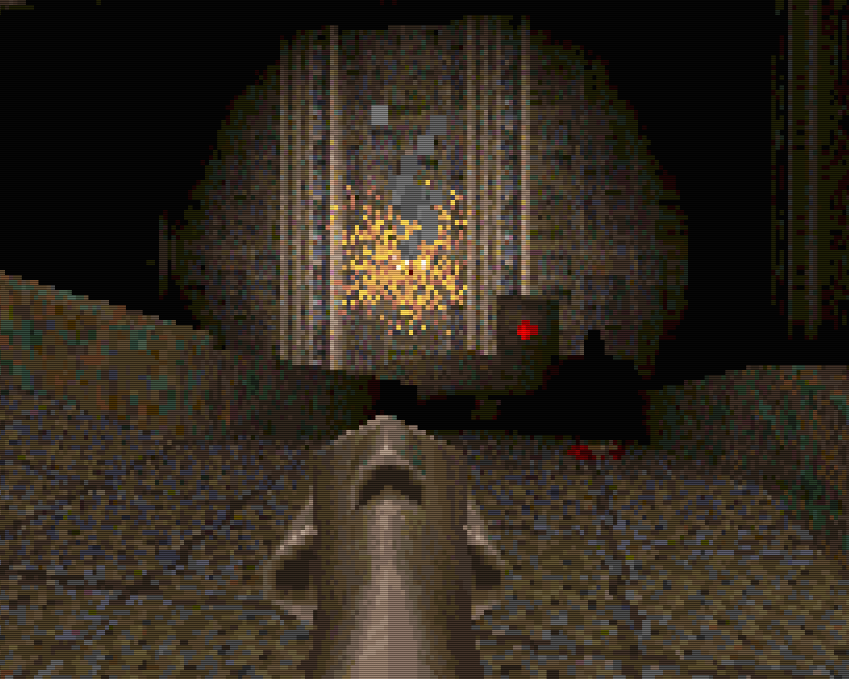
\includegraphics[width=\textwidth]{lightmap}
  \caption{L'impatto di un razzo proietta la sua luce con una lightmap}
  \label{fig:DOSBox Quake}
\end{subfigure}
\hfill
\begin{subfigure}[b]{0.49\textwidth}
  \centering 
  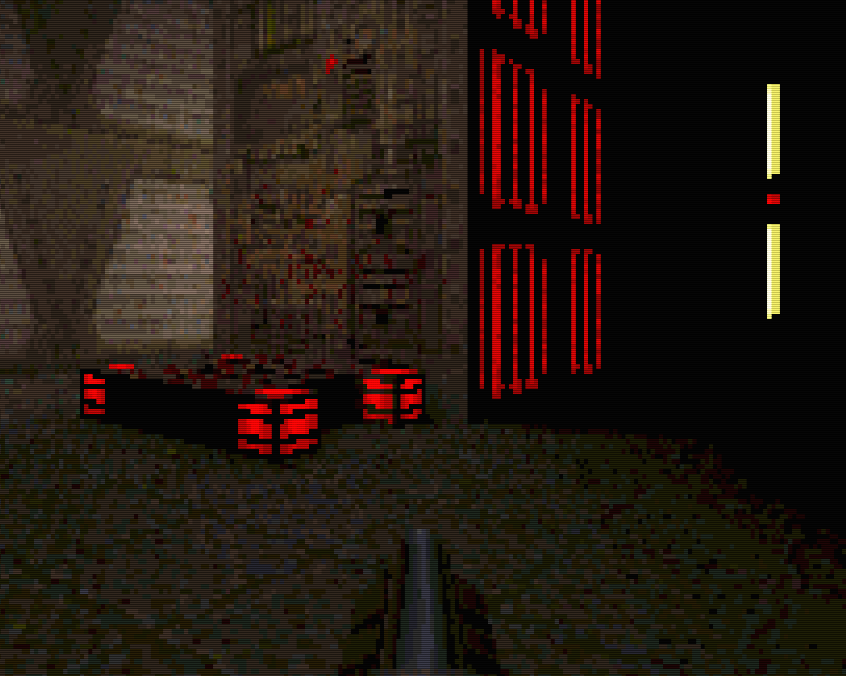
\includegraphics[width=\textwidth]{lightmap1}
  \caption{Sezione in ombra che mostra solo i pixel fullbright}
  \label{fig:Darkplaces Quake}
\end{subfigure}
\caption{Esempi di illuminazione}
\label{fig:Quake comparison}
\end{figure}

John Carmack implementò un'ottimizzazione ulteriore, la texture base e la lightmap di una superficie sono renderizzati allo stesso tempo, una ``surface cache'' memorizza nuove ``surfaces'', ovvero texture già illuminate che combinano la texture di base e le lightmap della mappa di gioco tramite un baking, le superfici non utilizzate per un numero di frame predefinito vengono poi eliminate e ne vengono create di nuove, generare queste superfici richiedeva meno tempo che un secondo lightning pass e risultò in un guadagno di performance notevole.

Tuttavia, data la limitatezza dell'hardware in termini di memoria, fu necessaria l'adozione di un meccanismo di MIP mapping. Questo approccio comporta la normalizzazione dei pixel delle texture in base alla loro distanza dalla camera. Ad esempio, una superficie prossima alla camera ha un rapporto texel a pixel di 1:1, mentre una superficie molto distante ha un rapporto di 1:4, con eventuali correzioni applicate attraverso tecniche come il box-filtering. Tali informazioni vengono memorizzate in tiles, pre-renderizzate e successivamente salvate su disco.

I modelli poligonali come mostri e giocatori vengono illuminati solo con una luce ambientale e una luce fissa distante, entrambe dipendono dal livello di illuminazione del pavimento su cui si trova l'entità.

\begin{figure}[h]
  \centering
  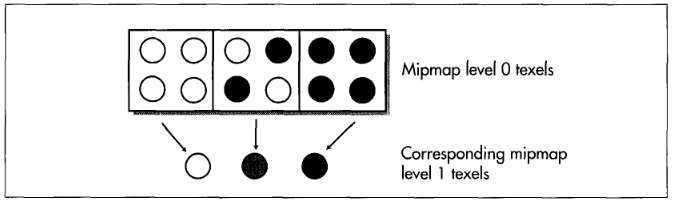
\includegraphics[width=\textwidth]{mipmapping}
  \caption{Come il MIP mapping riduce lo spazio nella cache \cite{abrash1997michael}}
  \label{fig:Texture diff in quakes}
\end{figure}

\section{Hardware Renderer}

%SISTEMARE QUESTA PARTE :TODO:
Inizialmente, Quake venne rilasciato per MS-DOS e presentava esclusivamente l'accelerazione grafica software, tuttavia con l'introduzione del motore VQuake, sviluppato sempre da John Carmack, il gioco fu uno dei prima a supportare le schede grafiche Rendition Vérité, che facevano uso di software proprietario e per cui era abbastanza complicato sviluppare. In seguito con il rilascio di GLQuake diventò possibile eseguire Quake tutte le schede grafiche compatibili con OpenGL. Altre versioni rilevanti includono WinQuake per Windows 95 e QuakeWorld.

Il codice sorgente di Quake, disponibile sulla pagina GitHub ufficiale, include tre diverse source port che utilizzano il rendering con accelerazione hardware tramite OpenGL. Nonostante ciò la versione WinQuake offre anche la possibilità di avviare il gioco utilizzando il software renderer su sitemi operativi Windows moderni. \cite{idsoftware:quake}

\subsection{Analisi del codice sorgente}

Nel 1997 venne rilasciato Quake World, una versione di Quake destinata prevalentemente al multiplayer in LAN o via Internet e che implementa diverse ottimizzazioni e ha come fondamento il codice di GLQuake.

La versione di OpenGL su cui si basa Quake World è la 1.0, di conseguenza il gioco utilizza una pipeline di rendering fixed-function e funziona in immediate-mode.

È possibile riassumere il game loop del lato client di Quake World come segue: 
\newline
\begin{lstlisting}[numbers=none,caption= Riassunto del main loop del client \cite{sanglard2013quake}]
WinMain
    while (1){
      newtime = Sys_DoubleTime ();
      time = newtime - oldtime;
      Host_Frame (time)
      {
        setjmp
        Sys_SendKeyEvents
        IN_Commands
        Cbuf_Execute
        /* Network */
        CL_ReadPackets
        CL_SendCmd
        /* Prediction/Collision */
        CL_SetUpPlayerPrediction(false)
        CL_PredictMove
        CL_SetUpPlayerPrediction(true)
        CL_EmitEntities
        /* Rendition */
        SCR_UpdateScreen
      }
    \end{lstlisting}

    Inizialmente, il client legge e processa tutti i messaggi e gli eventi inviati dal server. Successivamente, calcola le predizioni per i movimenti di tutte le entità del gioco e infine esegue il rendering dei modelli 3D della scena, aggiornando la visualizzazione per riflettere lo stato attuale del mondo e le azioni delle entità.
    
Il file header che contiene la definizione di tutti i prototipi delle funzioni di rendering è \texttt{render.h}, mentre i file che contengono le funzioni utilizzate nel rendering sono tutti quelli il cui nome ha come prefisso \texttt{r\_*}, i file che hanno come prefisso \texttt{gl\_*} sono invece le funzioni che utilizzano OpenGL. \cite{idsoftware:quake}

Il processo di rendering parte dalla funzione \texttt{SCR\_UpdateScreen} ed è possibile trovare la definizione di questa funzione nel file \texttt{gl\_screen.h}.

Il codice relativo al rendering può essere riassunto in questo modo: \newline

\begin{lstlisting}[  caption=SCR\_UpdateScreen \cite{sanglard2013quake},numbers=none]
SCR_UpdateScreen 		
{ 
	GL_BeginRendering
	SCR_SetUpToDrawConsole
	V_RenderView
	|	R_Clear
	|	R_RenderScene
	|	|	R_SetupFrame
	|	|		Mod_PointInLeaf
        |	|	R_SetFrustum
	|	|	R_SetupGL
	|	|	R_MarkLeaves
	|	|	|	Mod_LeafPVS
	|	|	|		Mod_DecompressVis
	|	|	R_DrawWorld
	|	|	|	R_RecursiveWorldNode
	|	|	|	DrawTextureChains
	|	|	|	|	R_RenderBrushPoly
	|	|	|	|		DrawGLPoly
	|	|	|	R_BlendLightmaps
	|	|	S_ExtraUpdate
	|	|	R_DrawEntitiesOnList
	|	|	GL_DisableMultitexture
	|	|	R_RenderDlights
	|	|	R_DrawParticles
	|	R_DrawViewModel
	|		R_DrawAliasModel
	|	R_DrawWaterSurfaces
	|	R_PolyBlend
	GL_Set2D
	SCR_TileClear
	V_UpdatePalette
	GL_EndRendering
}
\end{lstlisting}

In generale le prime funzioni chiamate sono:
\begin{enumerate}
\item \texttt{GL\_BeginRendering} Imposta le variabili (glx, gly, glwidth, glheight) successivamente utilizzate da \texttt{R\_SetupGL} per definire la viewport e la projection matrix
\item \texttt{SCR\_SetUpToDrawConsole} Decide l'altezza della console dei comandi in-game
\item \texttt{V\_RenderView} Renderizza la scena 3D
\item \texttt{GL\_Set2D} Cambia il tipo di proiezione rendendola ortografica (2D) per disegnare gli elementi 2D.
\item \texttt{SCR\_TileClear} Ripete una texture tramite tiling per riempire lo schermo intorno se la risoluzione selezionata è di dimensione inferiore.
\item \texttt{V\_UpdatePalette} Imposta la blending mode in base al danno ricevuto o al bonus attivo rendendo lo schermo colorato o più luminoso
\item \texttt{GL\_EndRendering} Cambia il buffer per il double-buffering
\end{enumerate}

All'interno di \texttt{V\_RenderView} vengono chiamate tre funzioni:
\begin{enumerate}
\item \texttt{V\_CalcRefdef} Esegue calcoli per la posizione del modello dell'arma, controlla la view height della camera ad esempio per simulare la camminata o quando il personaggio muore
\item \texttt{R\_PushDlights} Chiama la funzione ricorsiva di visita Front-To-Back dell'albero BSP \texttt{R\_MarkLights} rispetto ad ogni sorgente luminosa per marchiare i poligoni con tutte le luci che li riguardano.
\item \texttt{R\_RenderView}
\end{enumerate}


\texttt{R\_RenderView} a sua volta chiama:
\begin{enumerate}
\item \texttt{R\_Clear} Svuota i buffer GL\_COLOR\_BUFFER\_BIT e o GL\_DEPTH\_BUFFER\_BIT
\item \texttt{R\_RenderScene} 
\item \texttt{R\_DrawViewModel} Renderizza il giocatore in caso si trova in modalità spettatore
\item \texttt{R\_DrawWaterSurfaces} Cambia modalità a GL\_BLEND/GL\_MODULATE per dare l'effetto ondulato all'acqua (accede alle funzioni seno e coseno tramite una lookup table in \texttt{gl\_warp.c})
\item \texttt{R\_PolyBlend} Si occupa del blending impostato in \texttt{V\_UpdatePalette}
\end{enumerate}

\texttt{R\_RenderScene} chiama le funzioni più importanti:
\begin{enumerate}
\item \texttt{R\_SetupFrame} Ricava la foglia dell'albero BSP in cui si trova la camera.
\item \texttt{R\_SetFrustrum} Imposta il frustum \texttt{mplane\_t frustum[4]}
\item \texttt{R\_SetupGL} Imposta GL\_PROJECTION, GL\_MODELVIEW, viewport e glCullFace e ruota gli assi Z e Y siccome in Quake sono invertiti rispetto a OpenGL
\item \texttt{R\_MarkLeaves} Decomprime il Potentially Visible Set e itera per marchiare i nodi potenzialmente visibili
\item \texttt{R\_DrawWorld} Disegna il mondo percorrendo l'albero BSP Front-To-Back
\item \texttt{R\_ExtraUpdate} Resetta la posizione del mouse e si occupa di problemi con il cutoff dei suoni
\item \texttt{R\_DrawEntitiesOnList} Disegna modelli, brush e sprites
\item \texttt{GL\_DisableMultitexture} 
\item \texttt{R\_RenderDlights} Renderizza effetti di luce
\item \texttt{R\_DrawParticles} Disegna le particelle per esplosioni, fuoco, etc...
  \end{enumerate}
  \cite{sanglard2013quake}

Notare che non viene chiamata \texttt{GL\_LIGHTING} in quanto l'illuminazione viene comunque calcolata dalla CPU siccome avrebbe comunque utilizzato il Gouraud shading, ma in tempo reale invece che utilizzare le informazioni pre-compilate.
  
\subsection{Differenze con il renderer software}

Il codice relativo al rendering software può essere riassunto in questo modo:

\begin{lstlisting}[  caption=R\_RenderScene in \emph{r\_main.c} \cite{idsoftware:quake},numbers=none]
  R_RenderView
  | R_SetupFrame
  | | R_CheckVariables
  | | R_AnimateLight
  | | R_ViewChanged
  | | R_TransformFrustum
  | | D_SetupFrame
  | R_MarkLeaves
  | R_EdgeDrawing
  | | R_BeginEdgeFrame
  | | R_RenderWorld
  | | D_TurnZOn
  | | R_ScanEdges
  | R_DrawEntitiesOnList
  | | R_AliasDrawModel
  | | R_DrawSprite
  | R_DrawViewModel
  | R_DrawParticles
  
\end{lstlisting}

La differenza principale nel renderer software sta nella mancanza della funzione \texttt{R\_RenderScene} la quale utilizza le chiamate a OpenGL per il rendering del mondo utilizzando la pipeline della scheda grafica, in questo modo è presente molto overdraw che però non impatta sulle performance siccome i calcoli sono eseguiti da hardware specializzato, infatti utilizza il Z-Buffer per ogni operazione di hidden surface removal a livello di immagine. Al suo posto il codice originale implementa i meccanismi descritti nella sezione \ref{vsd}.

Un'altra differenza consiste nella gestione di texture e lightmaps, le quali sono gestite interamente dalla scheda grafica tramite il multitexturing, ovvero l'assegnazione di più texture ad una stessa superficie, in questo modo è possibile mantenere in memoria separatamente i dati riguardanti la luce e i dati riguardanti il colore della texture, inoltre permetteva di utilizzare lightmaps con colori RGB, aprendo la possibilità per l'illuminamento colorato che venne implementato con l'uscita di Quake 2.

La versione OpenGL ufficiale di Quake introduce diverse differenze visive rispetto all'originale. Una delle più evidenti è il texture filtering applicato da GLQuake, che rende le texture più lisce e smussate, ma a scapito dei dettagli originali. I tipi di filtering disponibili variano a seconda dell'hardware grafico ed è possibile modificare o disabilitare questa funzione tramite il comando in-game \texttt{gl\_texturemode}.

Un altro elemento estetico differente è la mancanza degli \texttt{overbrights}, l'engine originale consentiva alle lightmaps di raggiungere un livello di luminosità fino al 200\%, cosa che l'engine GLQuake non implementa. Inoltre nei livelli del gioco sono presenti texture con alcuni pixel che hanno luminosità massima indipendentemente dal contesto, perché il loro colore è codificato per ignorare le lightmaps. Poiché OpenGL gestisce l'illuminazione in modo diverso e non utilizza le colormaps, questi pixel non vengono mostrati in modo coerente con l'idea originale.

Inoltre per quanto riguarda le texture, l'engine software non corregge la distorsione delle texture presenti sui modelli 3D delle entità come mostri e armi, presumibilmente per motivi di performance, è possibile riabilitare questo effetto in GlQuake tramite il comando \texttt{gl\_affinemodels}.\cite{quaddicted2011swvsgl}

\begin{figure}[H]
  \centering
  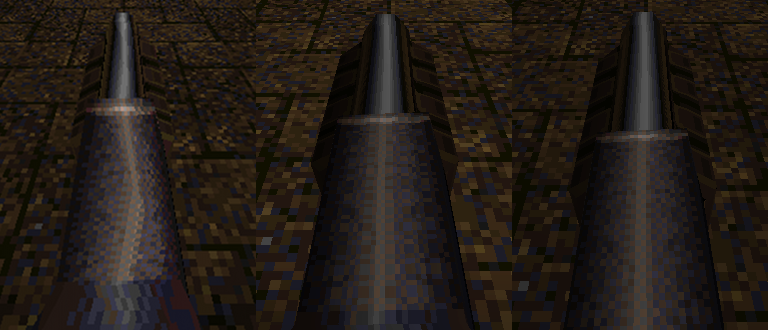
\includegraphics[width=\textwidth]{texturedistortion}
  \caption{Errori di texture (da sinistra a destra): Rendering Software, GLQuake e un engine moderno}
  \label{fig:Texture diff in quakes}
\end{figure}
\section{Conclusione}

Nonostante siano passati quasi 30 anni dall'uscita di Quake e l'hardware attuale permette di dare meno importanza a certe ottimizzazioni, lo studio di come si è arrivati alle tecniche utilizzate oggi è utile sia per prendere ispirazione dal passato che per comprendere le necessità che hanno portato a questo progresso, ciò non sarebbe possibile se non fosse stato rilasciato pubblicamente il codice sorgente del gioco e non esistessero archivi che si occupano di mantenere queste informazioni per le generazioni future.

``In a way, that’s frustrating, but the truth is, it’s these nearly-infinite possibilities that make 3-D so interesting; not only is it an endless varied challenge, but there’s almost always a better solution waiting to be found.''

- Michael Abrash \cite[Chapter~69]{abrash1997michael}

\newpage
\bibliographystyle{plain}
\bibliography{QuakeEngine}
\end{document}